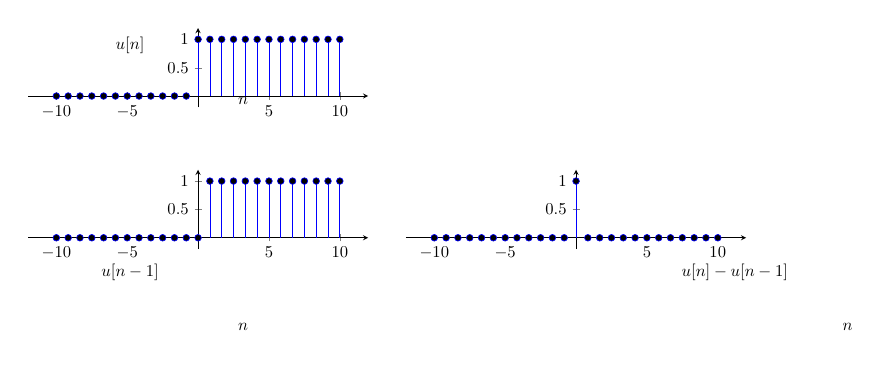
\begin{tikzpicture}[scale=0.6,
  declare function={
    unitstep(\x)= (\x>-0.1)*(1);
  },
    declare function={
    unitstepdelayed(\x)= (\x>0.1)*(1);
  },
    declare function={
    impulse(\x)= and(\x>-0.1, \x<0.1)*(1);
  }
]
\begin{axis}
[
    scale=1,
    axis x line=middle,
    axis y line=middle,
    every axis plot post/.style={mark options={fill=black}},
    xmin=-12,
    xmax=12,
    xlabel={$n$},
    ylabel={$u[n]$},
    y=1.2cm,
    x=0.3cm,
    ymin=-0.2,
    ymax=1.2,
        x label style={at={(current axis.right of origin)},anchor=west},
        y label style={at={(current axis.above origin)}, anchor=south},
]
%\addplot+[ycomb,blue] table [x={n}, y={xn}] {step.dat};
\addplot+[ycomb,domain=-10:10, blue] {unitstep(x)};
\end{axis}

\begin{scope}[yshift=-3cm]
	\begin{axis}
[
    scale=1,
    axis x line=middle,
    axis y line=middle,
    every axis plot post/.style={mark options={fill=black}},
    xmin=-12,
    xmax=12,
    xlabel={$n$},
    ylabel={$u[n-1]$},
    y=1.2cm,
    x=0.3cm,
    ymin=-0.2,
    ymax=1.2,
        x label style={at={(current axis.right of origin)},anchor=west},
        y label style={at={(current axis.above origin)}, anchor=south},
]
%\addplot+[ycomb,blue] table [x={n}, y={xn}] {step.dat};
\addplot+[ycomb,domain=-10:10, blue] {unitstepdelayed(x)};
\end{axis}
\end{scope}
\begin{scope}[xshift=8cm, yshift=-3cm]
	\begin{axis}
[
    scale=1,
    axis x line=middle,
    axis y line=middle,
    every axis plot post/.style={mark options={fill=black}},
    xmin=-12,
    xmax=12,
    xlabel={$n$},
    ylabel={$u[n] -u[n-1]$},
    y=1.2cm,
    x=0.3cm,
    ymin=-0.2,
    ymax=1.2,
        x label style={at={(current axis.right of origin)},anchor=west},
        y label style={at={(current axis.above origin)}, anchor=south},
]
%\addplot+[ycomb,blue] table [x={n}, y={xn}] {step.dat};
\addplot+[ycomb,domain=-10:10, blue] {impulse(x)};
\end{axis}
\end{scope}
\end{tikzpicture} 